\documentclass[12pt]{article}
\usepackage{graphicx}
\usepackage{amsmath}
\usepackage{amssymb}

\begin{document}

\begin{center}
{\large Review Set 3} 
\end{center}

This Review Set you to prepare written answers to questions on
context-free grammars and Earley parsers. 
Each of the questions has a short answer. You
may discuss this Review Set with other students and work on the
problems together.  

\begin{enumerate}

% #1
\item Use left-factoring and/or elimination of left recursion to convert
the following grammars into LL(1) grammars. You may assume that these
grammars are unambiguous.

\begin{enumerate}

\item

\begin{eqnarray*}
E & \rightarrow & E + T \ | \ T | \ E !\\
T & \rightarrow & int \ | \ ( E ) \\
\end{eqnarray*}

\item

\begin{eqnarray*}
L & \rightarrow & X \ | \ L , X  \\
X & \rightarrow & int \ | \ string \ | \ ( L ) \\
\end{eqnarray*}

\item

\begin{eqnarray*}
P & \rightarrow & P \ H \ 4 \ U \ | \ p \\
H & \rightarrow & h \\
U & \rightarrow & u \ | \ u \ P \\
\end{eqnarray*}

\end{enumerate}

% #2
\item 

Consider the following grammar:

\begin{eqnarray*}
  S & \rightarrow & A \\
  A & \rightarrow & A + A \ \ |\ \  B + + \hbox{\hskip 1in (Each '+' is a separate token.)}\\
  B & \rightarrow & y
\end{eqnarray*}

Draw the full Earley chart associated with parsing the input string \texttt{ y +
+ + y + + +} using the above grammar and indicate whether or not the Earley
parser accepts the string.

\item

In class we discussed how how to use Earley's algorithm to \emph{recognize}
if a string is in the language of a grammar. However, modern parsers can
do more than recognize: they can also produce parse trees, produce
derivations, or otherwise execute user-defined actions (as in \texttt{yacc} or
PA3) whenever a rewrite rule is applied. 

Explain in English prose how you would modify an Earley recognizer (such as
the one developed in the class notes and handouts) into a full-fledged
parser that executes user actions. Do not provide
code diffs or deltas. Instead, describe what additional information must be
maintained and how that information should be updated. Remember that 
user actions should be executed bottom-up even if the parsing algorithm is
top-down. Remember also that user actions can read values
associated with previously-executed rewrite rules (e.g., \texttt{\$\$ = new
PlusNode(\$1,\$3);} or \texttt{return new PlusNode(val[1], val[3]);} or the
like). 
Be precise: make it clear to the reader what data structures you
are adding or changing, how those data structures are updated, what
invariants are maintained, and when and in what order the user actions are
executed. 

\item

Consider an Earley parser, such as the one we discussed in class, with
the \emph{closure} (or \emph{predict}) operation removed. That is, this
new type of Parser only uses \emph{shift} (or \emph{scan}) and 
\emph{reduction} (or \emph{completion}) operations to fill in the chart of
parsing states. 
  \begin{itemize}
    \item Give a grammar $G_1$ and a string $S_1$ such that $S_1 \in
    L(G_1)$ but this new closure-less parser fails to recognize that $S_1$
    is 
    in $L(G_1)$. Explain why the parse fails in one sentence. 

    \item Give a grammar $G_2$ and a string $S_2$ such that $S_2 \in
    L(G_1)$ and this new closure-less parser still successfully recognizes
    that $S_2$ is in $L(G_2)$. 

  \end{itemize} 





\iffalse 
% #2
\medskip

\item Consider the following grammar fragment for a familiar syntax:

\begin{eqnarray*}
URL & \rightarrow & PROTO \ : \ / \ / \ HOST \ / \ FILE  \\
PROTO & \rightarrow & http \\
PROTO & \rightarrow & ftp \\
HOST & \rightarrow & id \ I \\
I & \rightarrow & \epsilon \\
I & \rightarrow & . \ HOST \\
FILE & \rightarrow & id \ G \\ 
G & \rightarrow & \epsilon \\ 
G & \rightarrow & . \ FILE \\
G & \rightarrow & / \ FILE \\
\end{eqnarray*}

The nonterminals are $URL$, $PROTO$, $HOST$, $I$, $FILE$ and $G$. 

\begin{enumerate}

\item Left-factor this grammar.

\item Give the First and Follow sets for each nonterminal in the grammar
obtained in part (a).

\item \label{lltable} Using this information, construct an LL parsing
table for the grammar obtained in part (a).

\item Suppose we generated an LL parser for the grammar using the table
you constructed. What would go wrong if it tried to parse the following
input string?

\[
ftp : / / id . id / id . / id . . id
\]

(That is, when we get an error, how much of the input string has been
consumed, and what is the parser trying to do?)

\end{enumerate}


% #3
\medskip

\item 

Consider the following LR(1) grammar:

\begin{eqnarray*}
  S & \rightarrow & A \\
  A & \rightarrow & A + A \ \ |\ \  B + + \hbox{\hskip 1in (Each '+' is a separate token.)}\\
  B & \rightarrow & y
\end{eqnarray*}

and its corresponding DFA:

\medskip
\begin{center}
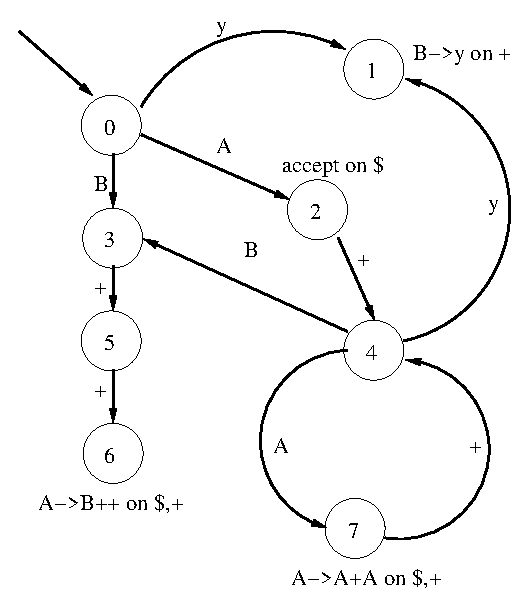
\includegraphics[bb=1.0in 0.0in 3.0in 4.0in]{rs3-diagram}
\end{center}
\medskip

Complete the table below, showing the trace of an LR(1) parser (which uses
the DFA above) on the input provided. The ``Stack'' column must show the
stack (with the top at right), the ``Input'' column shows the
not-yet-processed input terminals, and the ``Action'' column must show
whether the parser performs a shift action or a reduce action or accepts
the input. In the case of a reduce action, please indicate which
production is used.

\medskip
\begin{center}
\begin{tabular}{r@{\hspace{1cm}}l@{\hspace{2cm}}l}
Stack (with top at right) & Input & Action \\
\hline
      & $\blacktriangleright$ y + + + y + + + \$ & shift \\
    y &
\end{tabular}
\end{center}

\fi

\end{enumerate}

\end{document}
